\chapter{Padding Oracle攻击}

\section{实验目的}

理解 padding oracle 攻击的过程,验证攻击的可行性。

\section{实验准备}

网站 crypto-class.appspot.com 部署了一个填充预言机的模拟示例,请搭建
可以访问上述地址的实验环境。

\section{实验要求}

假设攻击者想要利用上述网站的返回结果窃取信息。攻击者通过观察得
知:网站将用户的数据加密后利用 URL 参数进行传输,例如:

\begin{center}
    http://crypto-class.appspot.com/po?er=f20bdba6ff29eed7b046d1df9fb7000
\end{center}

当用户 Alice 和网站进行交互时,网站将上述 URL 发送给 Alice。攻击者
猜测在"po?er="这一 URL 变量的值可能 Alice 会话中的一个一些秘密数据。该
数据使用 AES CBC(随机初始向量加密)模式进行加密并将加密结果使用
hex 进行编码。攻击者发现上述网站存在 padding oracle 攻击:当解密的
CBC 密文出现填充错误时,网站服务器返回 403 错误(forbidden request),
当 CBC 填充合法,但是 MAC 验证失败时,网站返回 404 错误(URL not 
found)。

请利用以上信息,解密上述代码框中的密文。为了完成解密,你可以发送
任意的如下格式的 HTTP 请求并获取其对用的错误代码。Padding oracle 可以
进行逐字节的解密,你需要发送 256 个 HTTP 请求来完成一个字节的解密。需
要注意的时密文的第一个分组是随机的初始向量,且解密得到的消息使用
ASCII 编码。

\begin{center}
    http://crypto-class.appspot.com/po?er=
\end{center}

\newpage
\section{实验内容}

\subsection{攻击方法分析}

如下图,为CBC模式下的解密示意图。

\begin{figure}[!htbp]
    \centering
    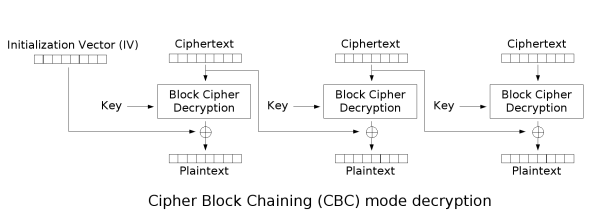
\includegraphics[width=0.9\textwidth]{cbc.png}
    \caption{CBC模式下的解密示意图}
\end{figure}
 
形式化的可以写为$P_i = D(K,C_i) \oplus C_{i-1}$,且有$C_0 = IV$。

在AES中,分块长度为16字节,当最后一块不够,或正好是16字节时,需要填充,规则为PKCS5。

此时,我们截获了密文$Y$,并想获得密文$Y$的最后一个字节。我们构造密文$F|Y$,那么服务器
在进行解密时,有$P=D(K,Y)\oplus F$,此时我们通过修改密文$F$的最后一个字节,$F_{15}$
就可以修改$Y$对应明文的最后一个字节。

给出对应的攻击过程:
\begin{enumerate}
    \item $i = 0$,$F$为随机字节
    \item $F_{15} = i \oplus 0x01$
    \item 将$F|Y$发送给服务器,若$P$的最后一个字节是$i$,则最后Padding为$0x01$,无错误,
    否则只有$P$最后$P_{15} \oplus i \oplus 0x01$字节都是$P_{15} \oplus i \oplus 0x01$
    才不会报错,此时满足的概率是小的,我们认为攻击成功。
    \item 若不满足,$i = i+1$,返回到第2步。
\end{enumerate}

当获取了最后一个字节,固定好后继续设置$F_{14}=i\oplus 0x02$就可继续获取倒数第二个字节,以此类推。

此处需要注意在猜测填充块(即最后一块)的倒数第一个字节时,若第3步不报错,需要修改IV的倒数第二个字节
打破填充规则,若此时仍然Padding正常,则说明猜测准确,否则需要继续猜测其他值。

(此处主要参考了CTF-Wiki中的攻击模式说明\footnote{https://ctf-wiki.org/crypto/blockcipher/mode/padding-oracle-attack})

\subsection{攻击结果}
由于实验环境特殊性,笔者根据mithi的工作\footnote{https://github.com/mithi/simple-cryptography/tree/master/04-padding-oracle}
在本地搭建了Padding Oracle攻击环境。

攻击结果:
\begin{lstlisting}
Case A
--------------
SERVER > localhost:9000
TARGET > 4ca00ff4c898d61e1edbf1800618fb2828a226d160dad07883d
04e008a7897ee2e4b7465d5290d0c0e6c6822236e1daafb94ffe0c5da05d
9476be028ad7c1d81
PLAINTEXT > Basic CBC mode encryption needs padding.
\end{lstlisting}